%
%     hw8_bbordwell.tex
%     Baylee Bordwell (baylee.bordwell@colorado.edu)
%     Based on the template by Benjamin Brown (bpbrown@colorado.edu)
%     Aug 27, 2014
%
%     Problem set 8 for ASTR/ATOC 5540, Mathematical Methods, taught at
%     University of Colorado, Boulder, Fall 2014.
%
%

\documentclass[10pt, preprint]{aastex}
% formatting based on 2014 NASA ATP proposal with Jeff Oishi

%%%%%%begin preamble
\usepackage[hmargin=1in, vmargin=1in]{geometry} % Margins
\usepackage{hyperref}
\usepackage{url}
\usepackage{times}
\usepackage{natbib}
\usepackage{graphicx}
\usepackage{amsmath}
\usepackage{amsfonts}
\usepackage{amssymb}
\usepackage{pdfpages}
\usepackage{import}
% for code import
\usepackage{listings}
\usepackage{color}
\usepackage{ragged2e}

\hypersetup{
     colorlinks   = true,
     citecolor     = gray,
     urlcolor       = blue
}

%% headers
\usepackage{fancyhdr}
\pagestyle{fancy}
\lhead{ASTR/ATOC 5540}
\chead{}
\rhead{name: Baylee Bordwell}
\lfoot{Problem Set 8}
\cfoot{\thepage}
\rfoot{Fall 2014}
% no hline under header
\renewcommand{\headrulewidth}{0pt}

\newcommand{\sol}{\ensuremath{\odot}}

% make lists compact
\usepackage{enumitem}
%\setlist{nosep}

%%%%%%end preamble


\begin{document}
\section*{Problem Set 8: Fourier transforms via FFTs and MMTs}
\begin{enumerate}
\item See Figure \ref{fig1}.
\begin{figure}[!ht]
\centering
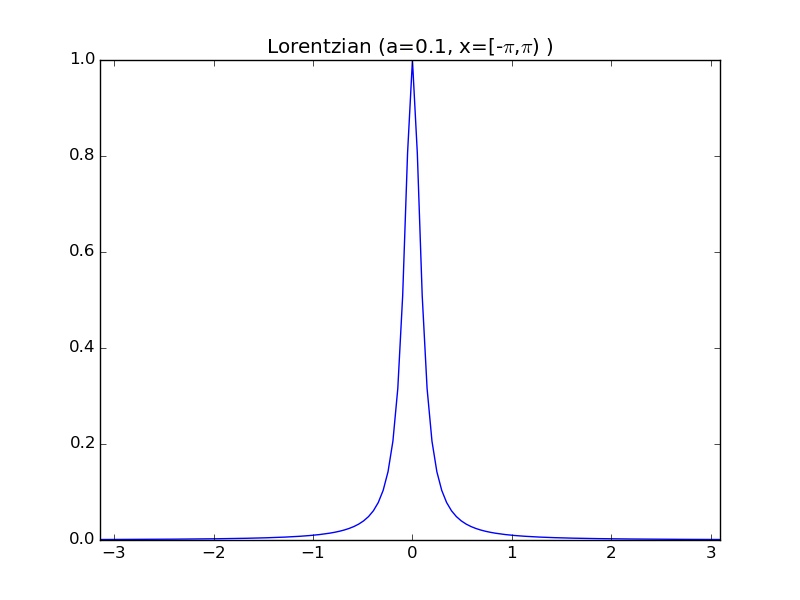
\includegraphics[width=3in]{hw8_fig1.png}
\caption{\centering \label{fig1}}
\end{figure}


\item Done.

\item As shown in Figure \ref{fig2}, power spectra from the MMT and the FFT are essentially indentical, with slightly increased error at higher frequencies. 
\begin{figure}[!ht]
\centering
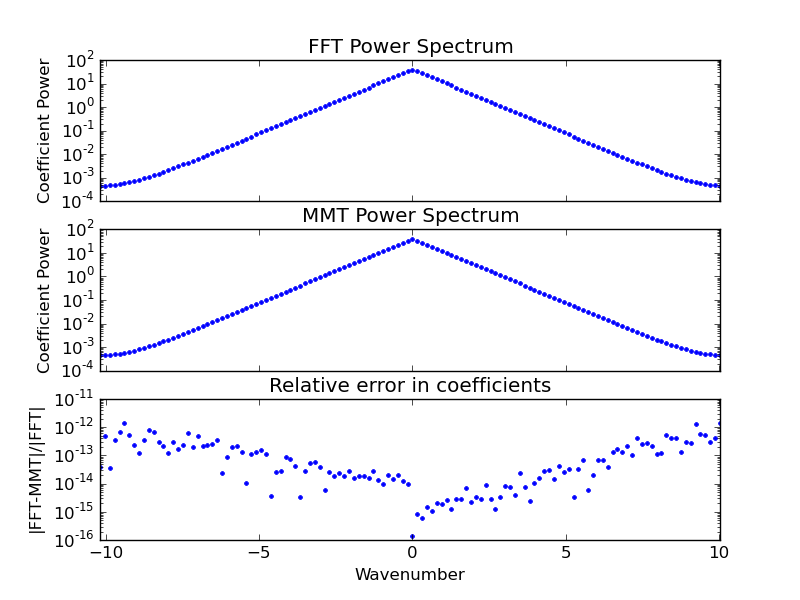
\includegraphics[width=5in]{hw8_fig2.png}
\caption{\centering \label{fig2}}
\end{figure}


\item The Lorentzian produced using the inverted MMT is virtually identical, as shown in the second plot in Figure \ref{fig3}. The top plot shows this similarity, with the inverted plot offset vertically to allow visual comparison.
\begin{figure}[!ht]
\centering
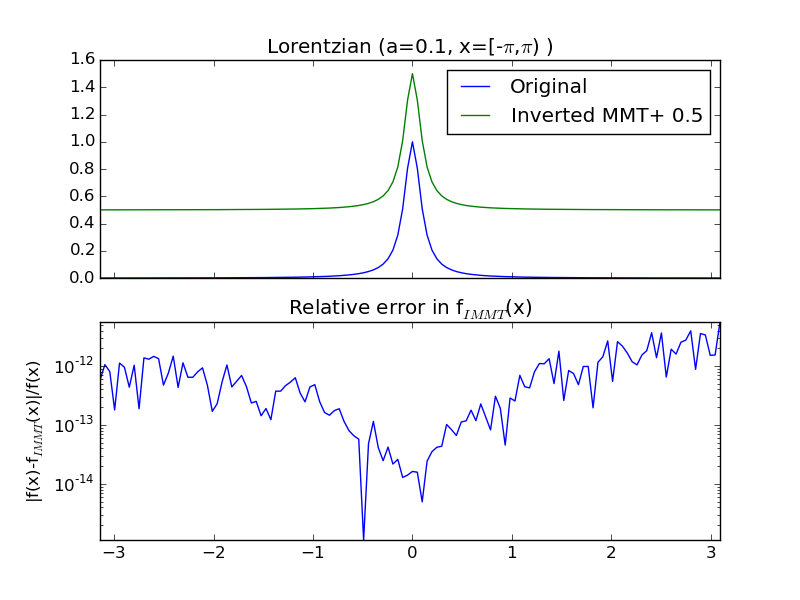
\includegraphics[width=4in]{hw8_fig3.png}
\caption{\centering \label{fig3}}
\end{figure}

\item For very low sample sizes, the MMT beats out the FFT, but generally the FFT will always win for sample sizes that are powers of 2, and the amount of lag it picks up over time grows more slowly than that of the MMT, as shown in Figure \ref{fig4}
\begin{figure}[!ht]
\centering
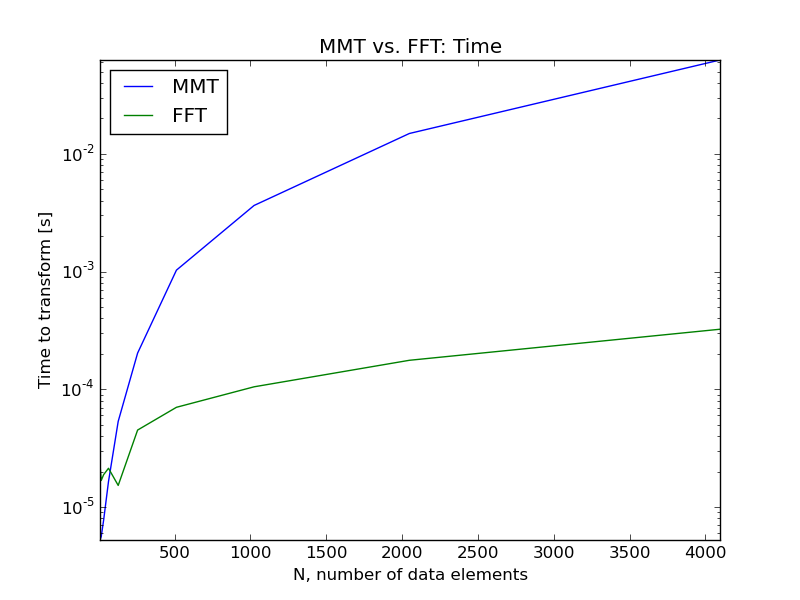
\includegraphics[width=3in]{hw8_fig4.png}
\caption{\centering \label{fig4}}
\end{figure}


\item As shown in Table \ref{tab1}, changing to a sample size that was not a power of 2 led to the FFT taking a much more similar amount of time to the MMT, dropping to only being about 6 times faster.
\begin{table}[!ht]
\centering
\begin{tabular}{c c c c}
  N & $t_{MMT}$ (s) & $t_{FFT}$ (s) & $t_{MMT}/t_{FFT}$\\
  \hline
  2048 & 1.4912$\cdot10^{-2}$ & 1.7643$\cdot10^{-4}$ & 84.519\\
  2049 & 1.5039$\cdot10^{-2}$ & 2.5755$\cdot10^{-3}$ & 5.8393\\
\end{tabular}
\caption{\centering \label{tab1}}
\end{table}
\end{enumerate}

Code used in this assignment can be found at \url{https://github.com/brbordwell/ASTR_5540/HW8}
\end{document}
